\documentclass{article}

\usepackage{listings}
\usepackage{enumitem}
\usepackage{amsmath}
\usepackage{svg}
\usepackage{hyperref}
\hypersetup{
    colorlinks=true,
    linkcolor=blue,
    filecolor=magenta,      
    urlcolor=cyan,
    pdftitle={Overleaf Example},
    pdfpagemode=FullScreen,
    }

\title{CA Lab: Lab 5}
\author{student: Dimitri Tabatadze}

\definecolor{codegreen}{rgb}{0,0.6,0}
\definecolor{codegray}{rgb}{0.5,0.5,0.5}
\definecolor{codepurple}{rgb}{0.58,0,0.82}
\definecolor{backcolour}{rgb}{0.98,0.96,0.94}

\lstdefinestyle{mystyle}{
    backgroundcolor=\color{backcolour},   
    commentstyle=\color{codegreen},
    keywordstyle=\color{magenta},
    numberstyle=\tiny\color{codegray},
    stringstyle=\color{codepurple},
    basicstyle=\ttfamily\footnotesize,
    breakatwhitespace=false,         
    breaklines=true,                 
    captionpos=b,                    
    keepspaces=true,                 
    numbers=left,                    
    numbersep=5pt,                  
    showspaces=false,                
    showstringspaces=false,
    showtabs=false,                  
    tabsize=2
}

\lstset{style=mystyle}

\begin{document}
    \maketitle

    \section*{Task Description} 
    
    \begin{enumerate}
        \item In the module file use always statement with case. (20 points)
        \item Write the testbench. (20 points)
        \item Use RTL viewer and show the drawing of 2-t0-4 decoder. (5 points)
        \item Simulate the testbench and make the analyze of timing diagram. (10 points)
        \item Run the code on the board. (40 points)
    \end{enumerate}

    \section*{Solution}
    
    \begin{enumerate}
        \item {
            The code:
            % \bf
            \begin{lstlisting}[language=verilog]
module decoder (
    input [1:0] in,
    output reg [3:0] out);

always @ (in)
begin
    case (in)
        2'b00 : out = 4'b0001;
        2'b01 : out = 4'b0010;
        2'b10 : out = 4'b0100;
        2'b11 : out = 4'b1000;
    endcase
end

endmodule\end{lstlisting}

            As you see, I have ommited the \verb|default| case, which is optional. In this case, the cases are exhaustive, so there's no point to having a default case --- it will never be entered.
        }
        \item {
            The code:
            \bf
            \begin{lstlisting}[language=verilog]
`include "decoder.v"

module decoder_tb();

reg [1:0] in;
wire [3:0] out;

decoder UUT(.in(in), .out(out));

initial begin
                                  // These two lines are
    $dumpfile("decoder_tb.vcd");  // used for logging
    $dumpvars(0, decoder_tb);     // the data, quartus
                                  // doesn't need them.
    in = 2'b00;
    #100;
    in = 2'b01;
    #100;
    in = 2'b10;
    #100;
    in = 2'b11;
    #100;
end

endmodule\end{lstlisting}
        }
        \item {
            I don't have quartus, but this is something that should be equivalent to what the RTL viewer would produce. I've give the schematic a test input of \ 01

            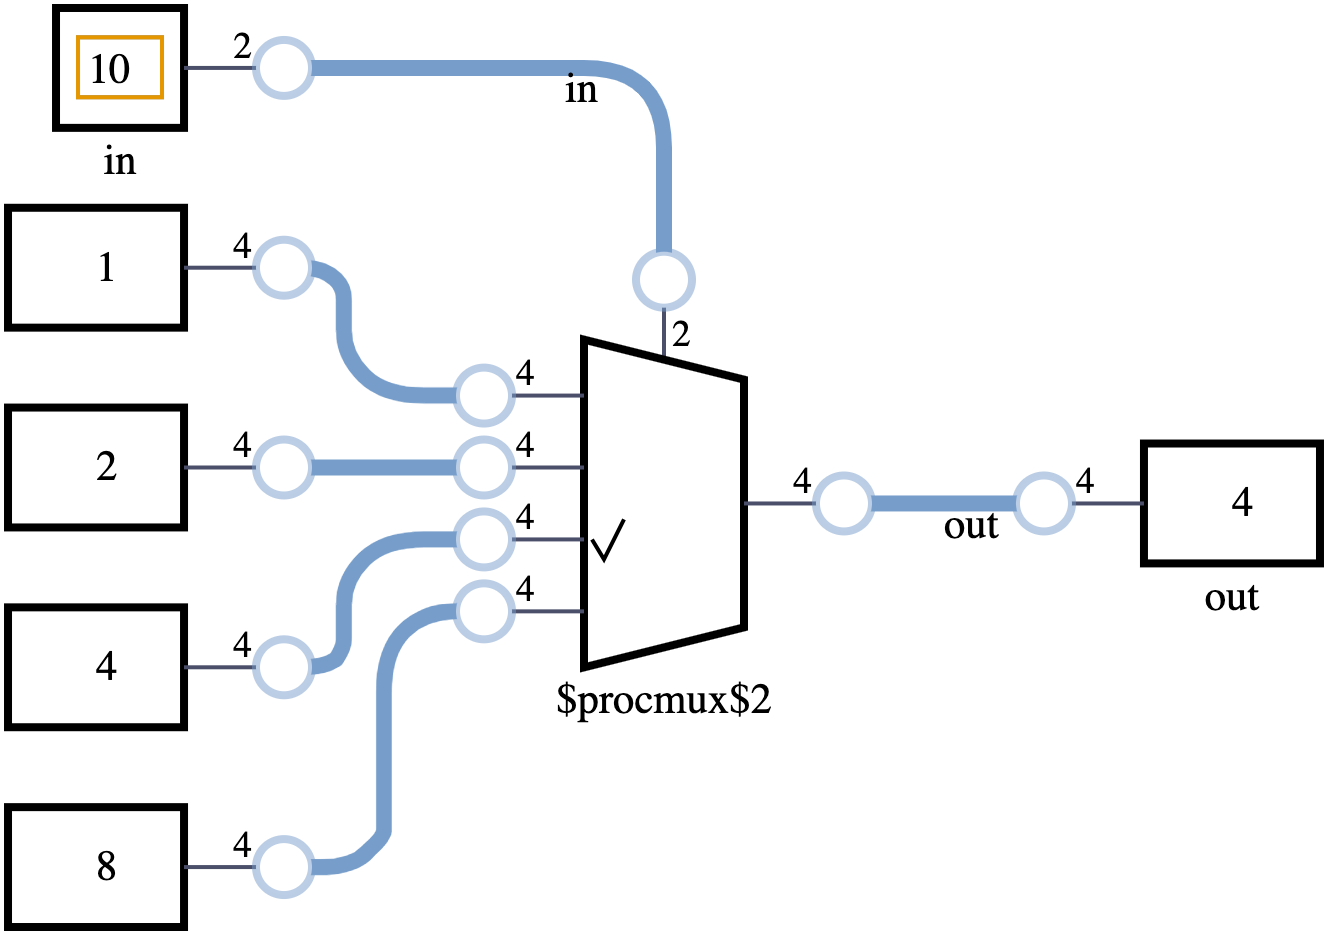
\includegraphics[width=10cm]{circuit.png}

            This visualization was made using \verb|DigitalJS| plugin for VSCodium.
        }
        \item {
            I used \verb|vvp| for simulation and \verb|GTKWave| for visualization. Here's the result:

            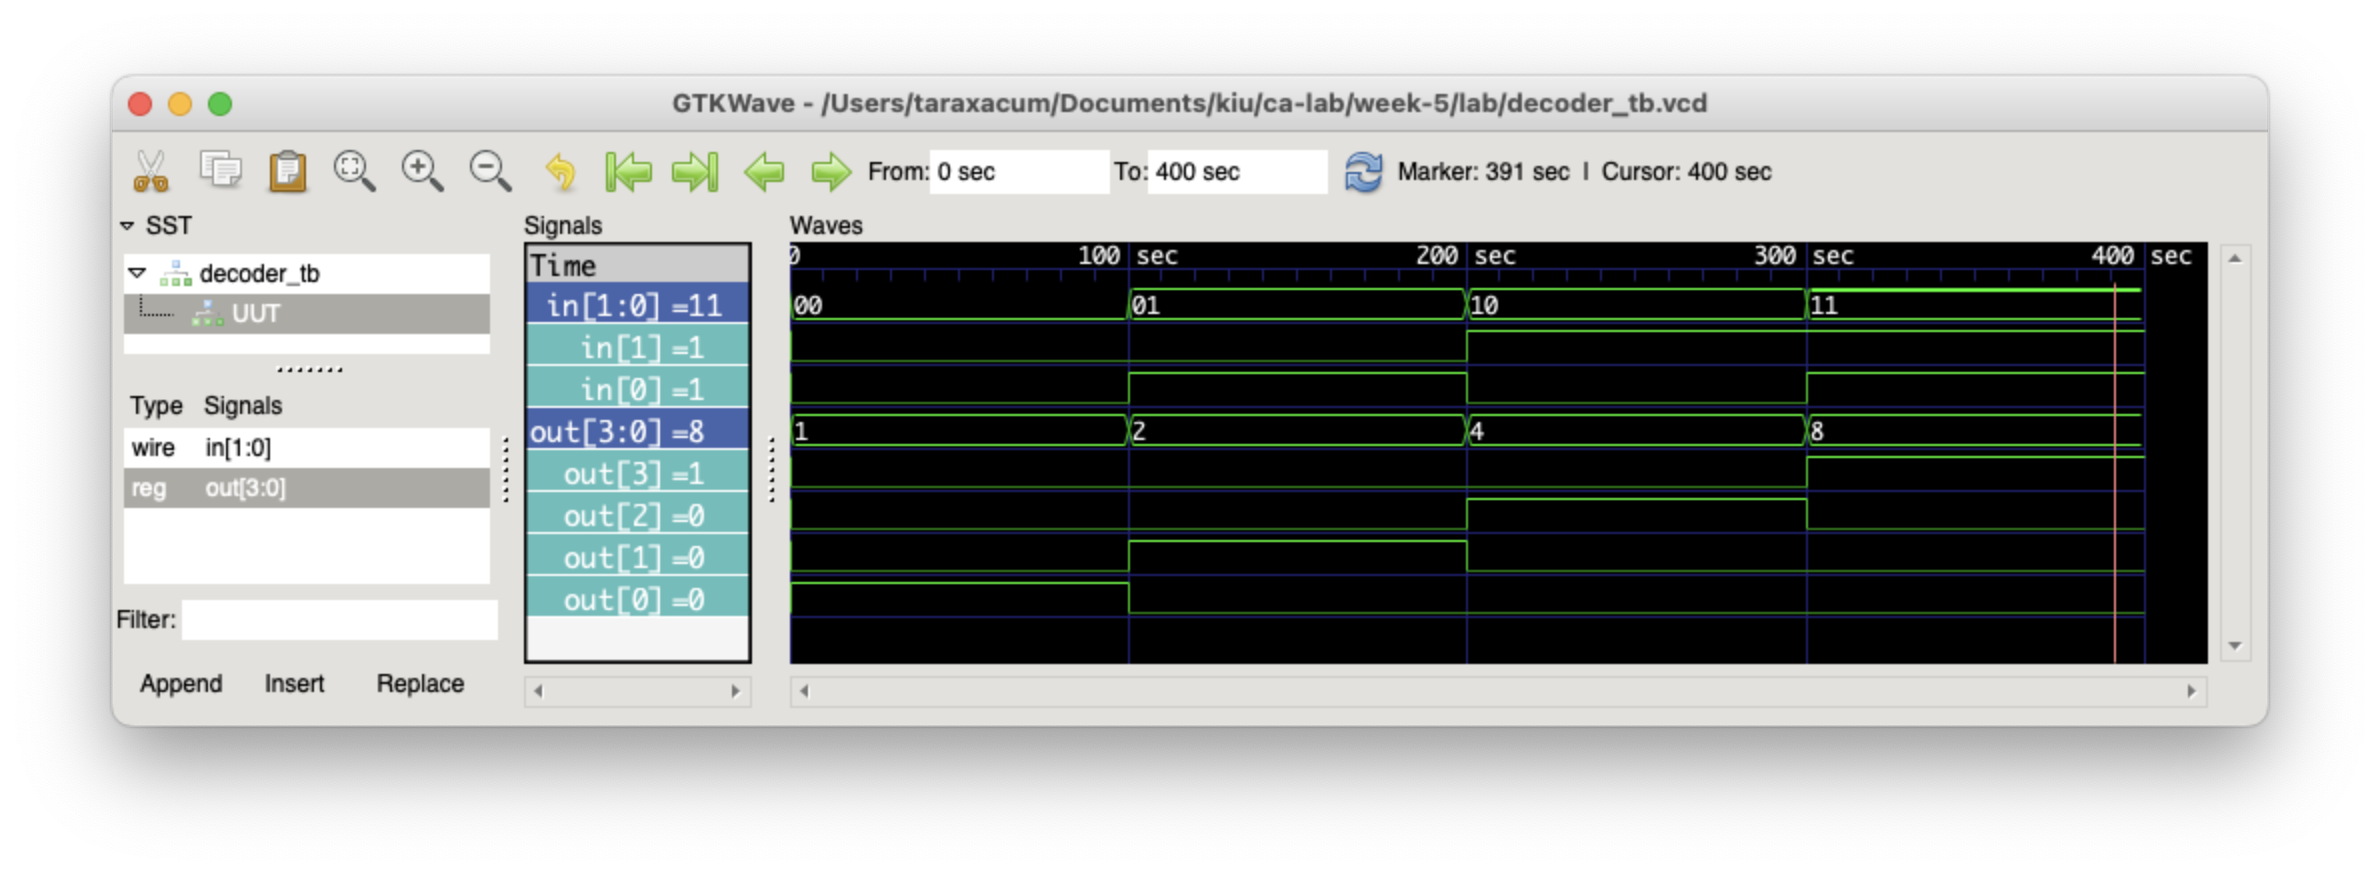
\includegraphics[width=11cm]{diagram.png}

            It's clear that the program is doing just what we wanted it to do. Given input \verb|11| (which is \(3\) in decimal), the 3-rd bit (counting from \(0\)) is set, while others are not.
        }
    \end{enumerate}

    \section*{Conclusion}
    
    Since I don't have the ability to run Quartus on my laptop and am using FOSS alternatives for doing everything I would have done with quartus, other than being able to run my code on physical hardware, I will be using a friend's laptop (or any laptop I can get a hold of which has quartus installed) to run my code on a board.

    \section*{Reference}
    
    \begin{itemize}
        \item \href{https://www.chipverify.com/verilog/verilog-always-block}{Where I learned about the always block}
        \item \href{https://www.chipverify.com/verilog/verilog-case-statement}{Where I learned about the case statement}
    \end{itemize}

\end{document}